
\documentclass[english, a4paper, 12pt]{article}
\usepackage[T1]{fontenc}
\usepackage[utf8]{inputenc}
\usepackage[english,francais]{babel}
\usepackage{fullpage}
\usepackage{color}
\usepackage{graphics, graphicx}
\usepackage{wrapfig}
\usepackage{natbib}
\usepackage{algorithm2e}
\usepackage{amsmath}
\usepackage{amssymb}
\usepackage{caption}
\usepackage{lineno}
\usepackage{changepage}
\usepackage{pifont}
\usepackage{wasysym}
\usepackage[dvipsnames]{xcolor}
\usepackage{nameref,hyperref}
\usepackage{bookmark}
\usepackage[babel=true]{csquotes}
\usepackage{setspace}

\usepackage{hyperref}
\hypersetup{
    backref=true,
    pagebackref=true,
    hyperindex=true,
    colorlinks=true,
    breaklinks=true,
    urlcolor=black,
    linkcolor=black,
    citecolor=black,
    bookmarks=true,
    bookmarksopen=true,
    pdffitwindow=true,
    pdfauthor={},
    pdftitle={},
    pdfsubject={},
    pdfcreator={},
    pdfkeywords={}
}

% Define environnement tablehere
\renewcommand{\textfraction}{0}
\makeatletter
\newenvironment{tablehere}
{\def\@captype{table}}
{}

% Define environnement figurehere
\newenvironment{figurehere}
{\def\@captype{figure}}
{}
\makeatother

\newcommand{\sigmaFGM}{$\sigma$\textsc{FGM}}

\title{Building the genetic map of \textit{Tribolium castaneum} from individual-level RNA-seq data}
\author{Charles Rocabert}
\date{}

\begin{document}
\selectlanguage{english} 

\maketitle

%\begin{figure}[!h]
%\begin{adjustwidth}{-0in}{0in}
%\centering
%\includegraphics[width=0.7\linewidth]{./taylor_mason.jpg}
%\end{adjustwidth}
%\end{figure}

\tableofcontents

%\thispagestyle{empty}

\newpage

%%%%%%%%%%%%%%%%%%%%%%%%%%%
\section{Introduction}

Individual RNA-seq data is derived from a population of \textit{Tribolium castaneum}, at the 1st and 21st generations of an experimental evolution protocol. The experiment comprises two environmental conditions (Control and Hot-Dry) with 4 replicates each (figure 1). For each of the four replicates, approximately 60 individuals have been sampled at generation 1, and approximately 16 at generation 21, leading to 614 samples (figure 2).

SNP detection was performed with GATK software on all RNA-seq samples.

\hfill

\begin{figurehere}
\centering
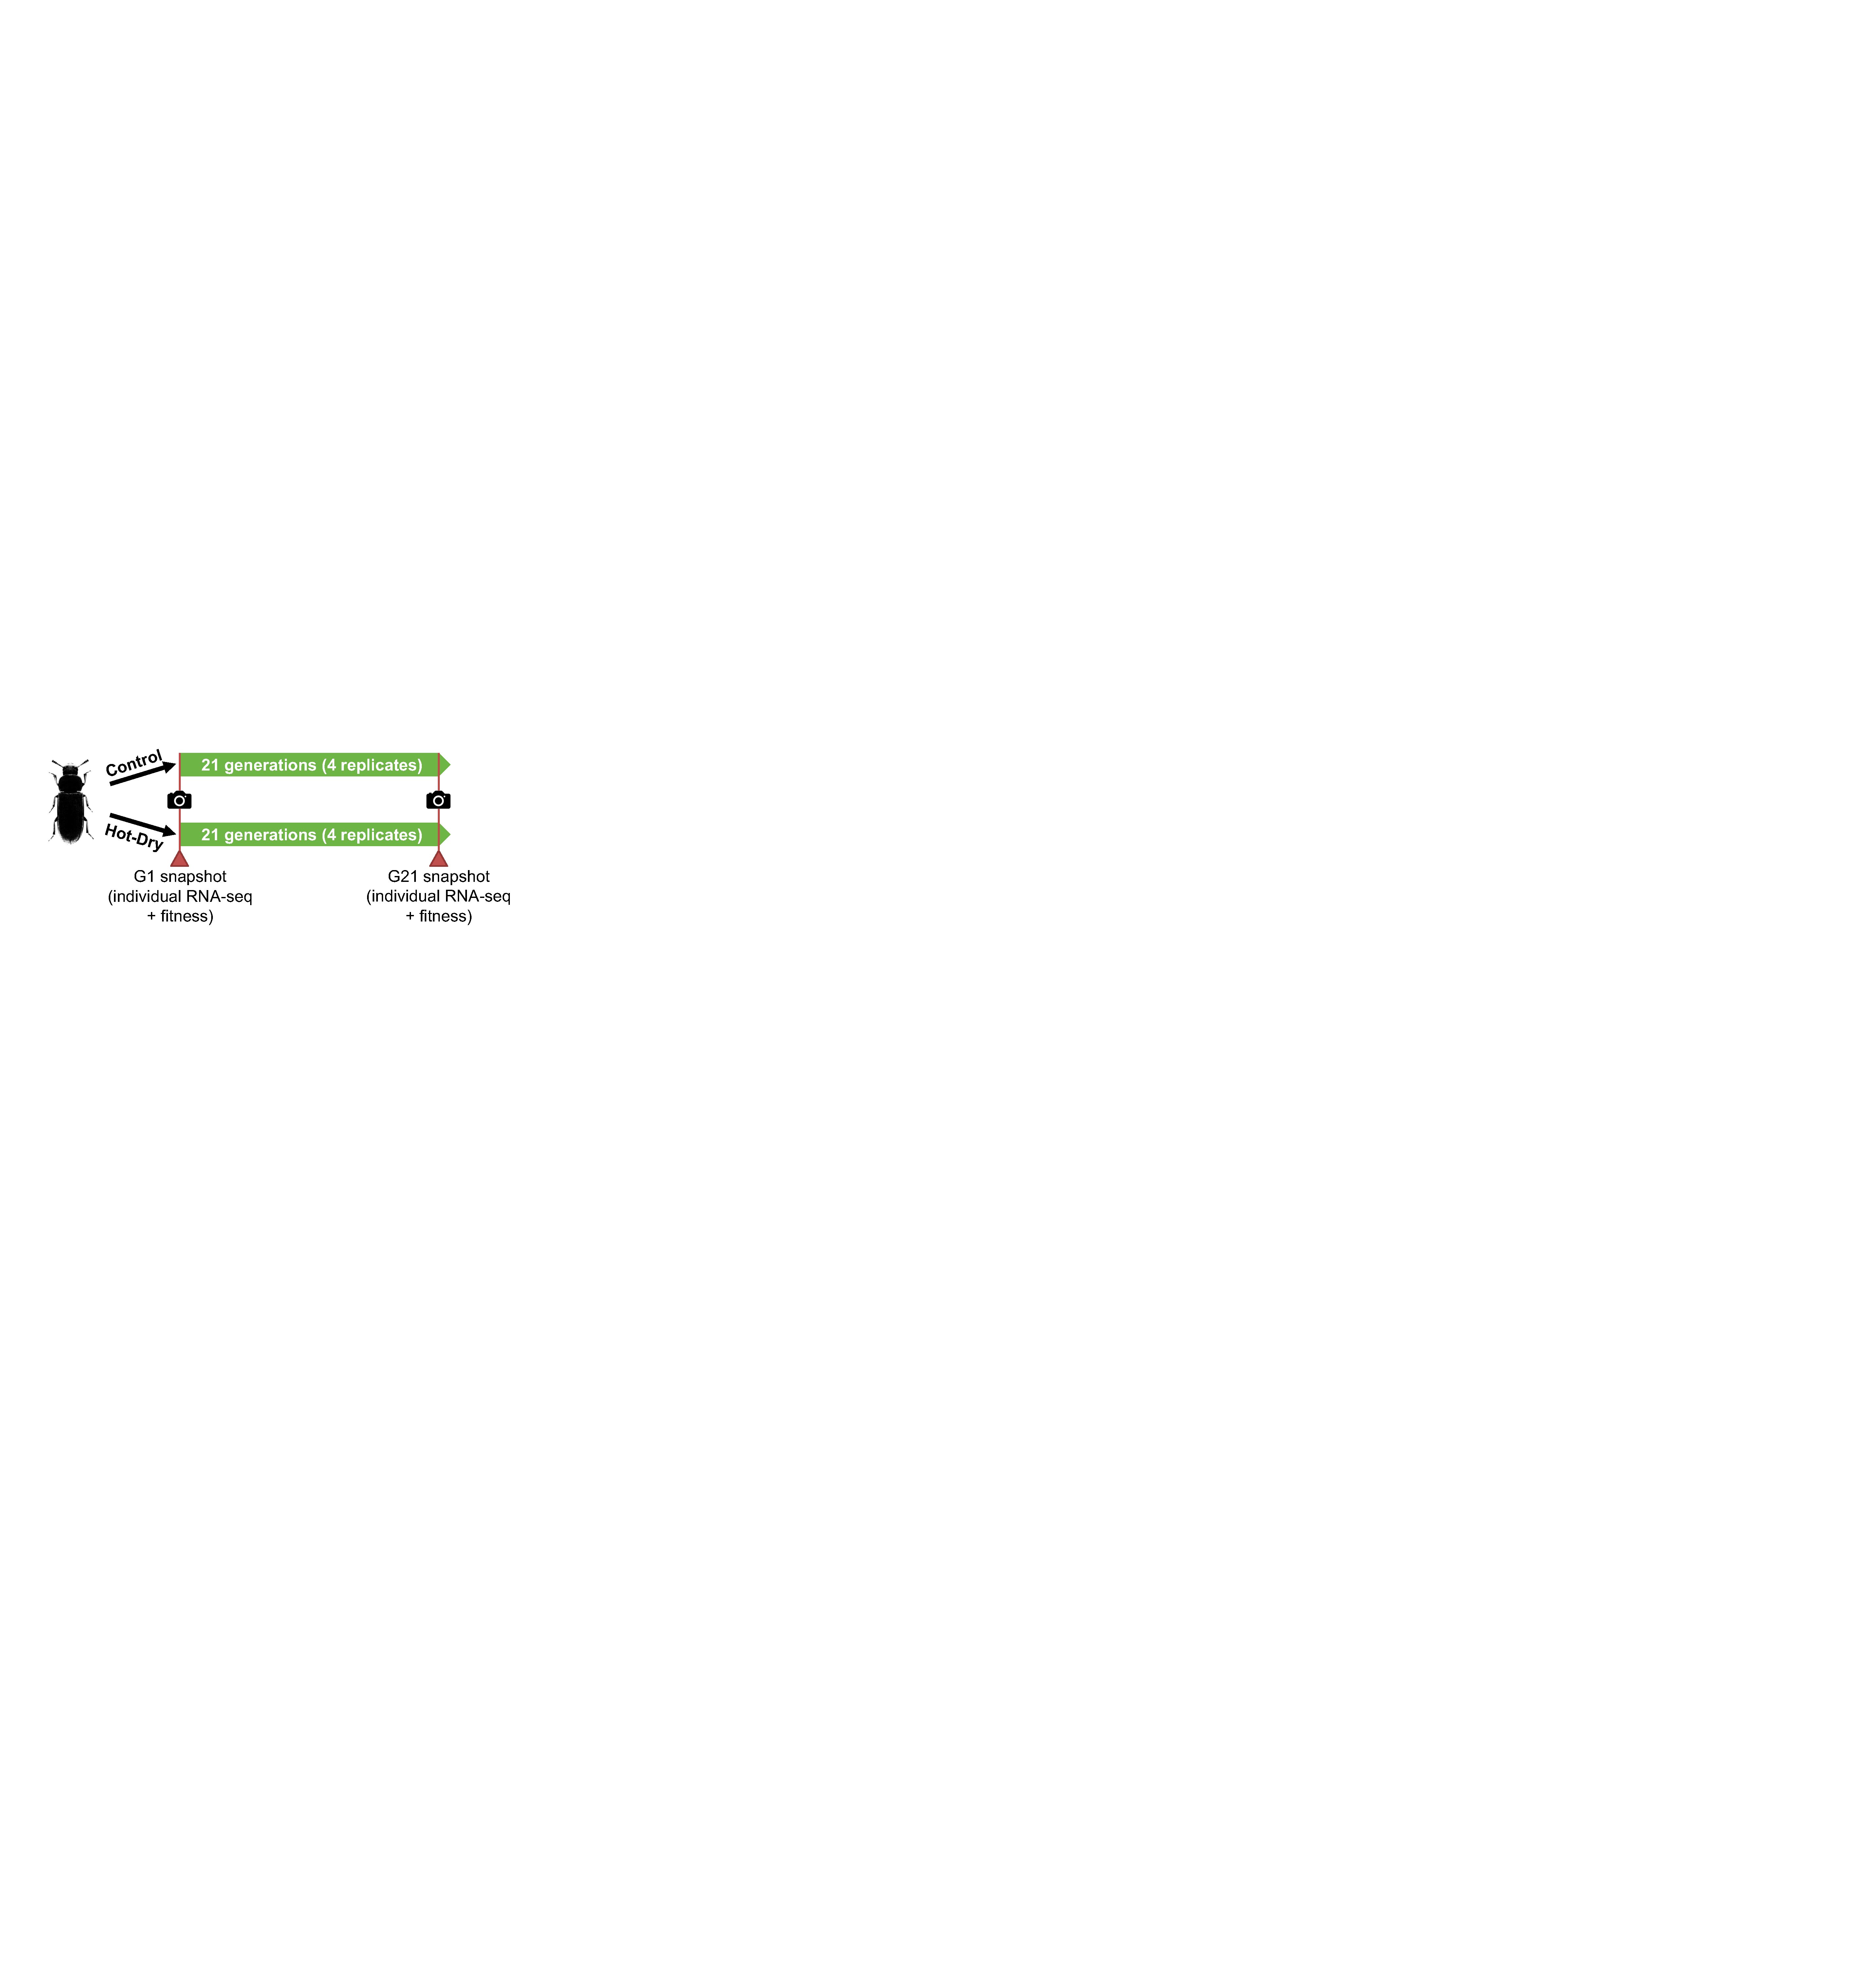
\includegraphics[width=0.6\linewidth]{figure1.pdf}
\caption{\small{A population of \textit{Tribolium castaneum} is placed under selection in two different environments (with 4 independent replicates each): Control, and Hot-Dry. At generations 1 and 21, individual RNA-seq samples and fitness measurements are performed.}}
\end{figurehere}

\hfill

\begin{figurehere}
\centering
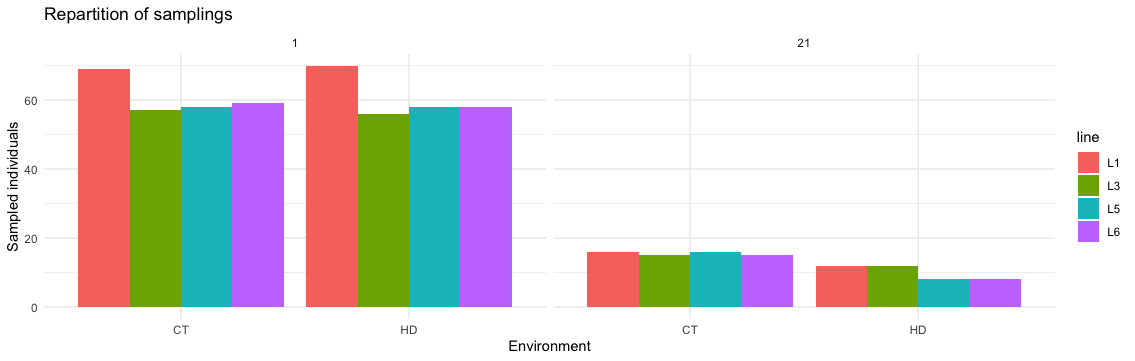
\includegraphics[width=1\linewidth]{figure1_bis.png}
\caption{\small{Repartition of samples by environment, line and generation.}}
\end{figurehere}

%%%%%%%%%%%%%%%%%%%%%%%%%%%
\section{Pipeline}

\subsection{Pre-processing}

Before calling Lep-MAP3 functions, a filtered VCF has been produced from the raw SNP call ($\text{DP}>=3$, $\text{F\_MISSING}<=0.5$, $\text{MAF}>0.0$), and a pedigree file containing father/mother relationships is produced (fathers and mothers are not part of the sampling).

\subsection{ParentCall2}

The function \texttt{ParentCall2} is called with the following parameters:
\begin{itemize}
\item \texttt{halfSibs = 1};
\item \texttt{removeNonInformative = 1};
\end{itemize}

\subsection{Filtering2}

The function \texttt{Filtering2} is called with the following parameters:
\begin{itemize}
\item \texttt{removeNonInformative = 1};
\item \texttt{dataTolerance = 0.01};
\end{itemize}

\subsection{LOD limit exploration to find the best chromosome separation}

The function \texttt{SeparateChromosomes2} is called with the following parameters:
\begin{itemize}
\item \texttt{lodLimit $\in \{5, 20\}$};
\item \texttt{distortionLod = 1};
\item \texttt{numThreads = 10};
\end{itemize}

To find the LOD limit leading to the best chromosome separation, \texttt{LODlimit} values have been explored in the range $\{5, 20\}$.
\textit{Tribolium castaneum} has 10 chromosomes, thus the most accurate chromosome separation is obtained with \texttt{LODlimit = 12} (figure 2).

\hfill

\begin{figurehere}
\centering
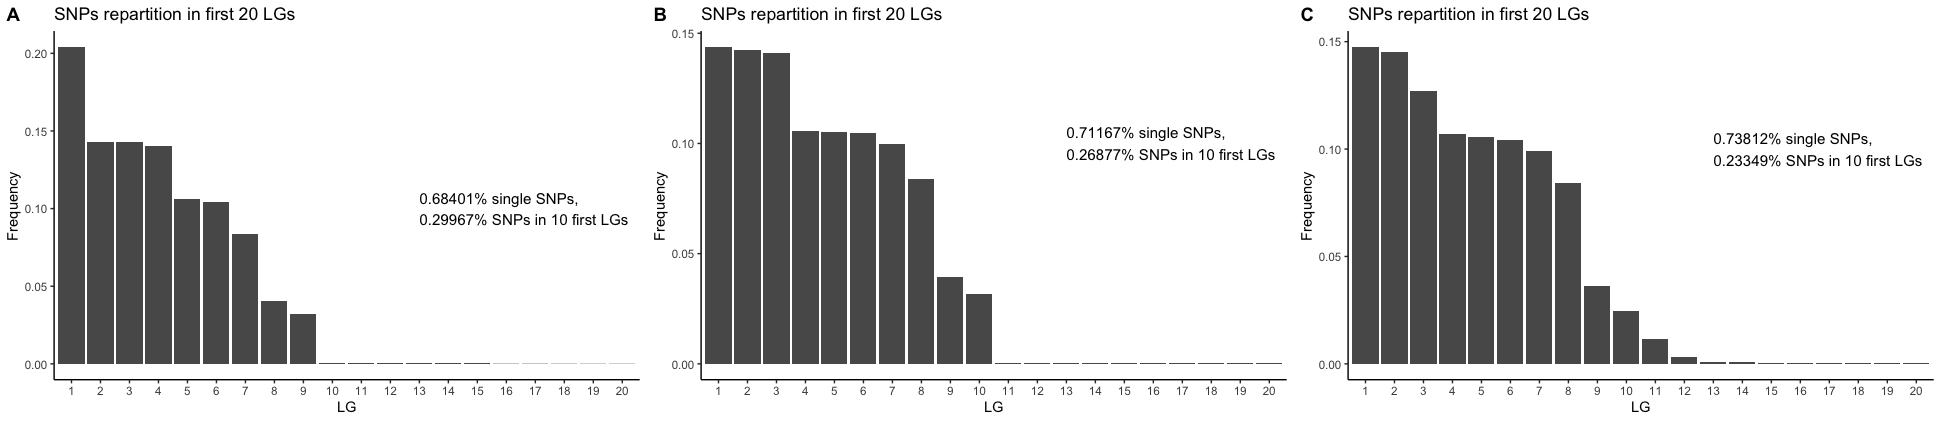
\includegraphics[width=1\linewidth]{figure2.png}
\caption{\small{Repartition of SNPs in the 20 first linkage groups. \textbf{(A)} \texttt{LODlimit = 11}. \textbf{(B)} \texttt{LODlimit = 12}. \textbf{(C)} \texttt{LODlimit = 13}}}
\end{figurehere}

\hfill

For \texttt{LODlimit = 12}, the repartition of SNPs in the 10 first linkage groups accurately matches the known repartition of SNPs in chromosomes (figure 3).

\hfill

\begin{figurehere}
\centering
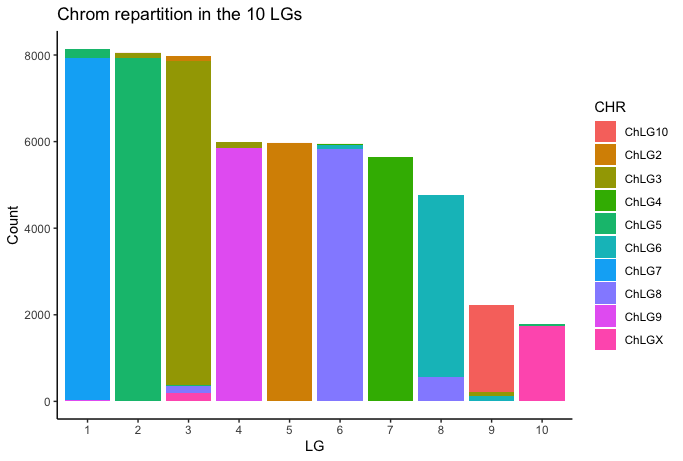
\includegraphics[width=0.5\linewidth]{figure3.png}
\caption{\small{Repartition of SNPs in the 10 first linkage groups. SNPs are colored by their known repartition in the 10 chromosomes of \textit{Tribolium castaneum}.}}
\end{figurehere}

\subsection{Manual reset of additional linkage groups}
All SNPs belonging to linkage groups > 10 are re-labelled to zero with an \textit{ad hoc} script (a SNP labelles to zero does not belong to any linkage group).

\subsection{JoinSingles2All}

The function \texttt{JoinSingles2All} is called with the following parameters:
\begin{itemize}
\item \texttt{lodLimit = 8};
\item \texttt{distortionLod = 1};
\item \texttt{iterate = 1};
\item \texttt{numThreads = 10};
\end{itemize}

This step adds 29,235 single SNPs to the first 10 linkage groups (51\% increase), leading to a total of 85,727 SNPs (figure 4).

\hfill

\begin{figurehere}
\centering
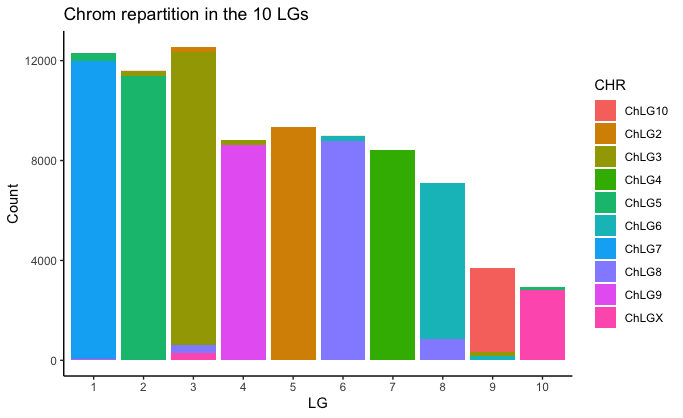
\includegraphics[width=0.5\linewidth]{figure4.png}
\caption{\small{Repartition of SNPs in the 10 first linkage groups after running Lep-MAP3 function \texttt{JoinSingles2All}. SNPs are colored by the known repartition in the 10 chromosomes of \textit{Tribolium castaneum}.}}
\end{figurehere}

\subsection{Manual cleaning of the map}

All single SNPs, as well as SNPs attributed to a linkage group but not belonging to the major chromosome of this group are removed with an \textit{ad hoc} script (for example in figure 4, the major chromosome of linkage group 1 is ChLG7).

After this step, the map is ready for markers sorting. The number of SNPs per linkage group correlates to known chromosome lengths (figure 5, adjusted $R^2=0.46$, p-value = 0.02).

\hfill

\begin{figurehere}
\centering
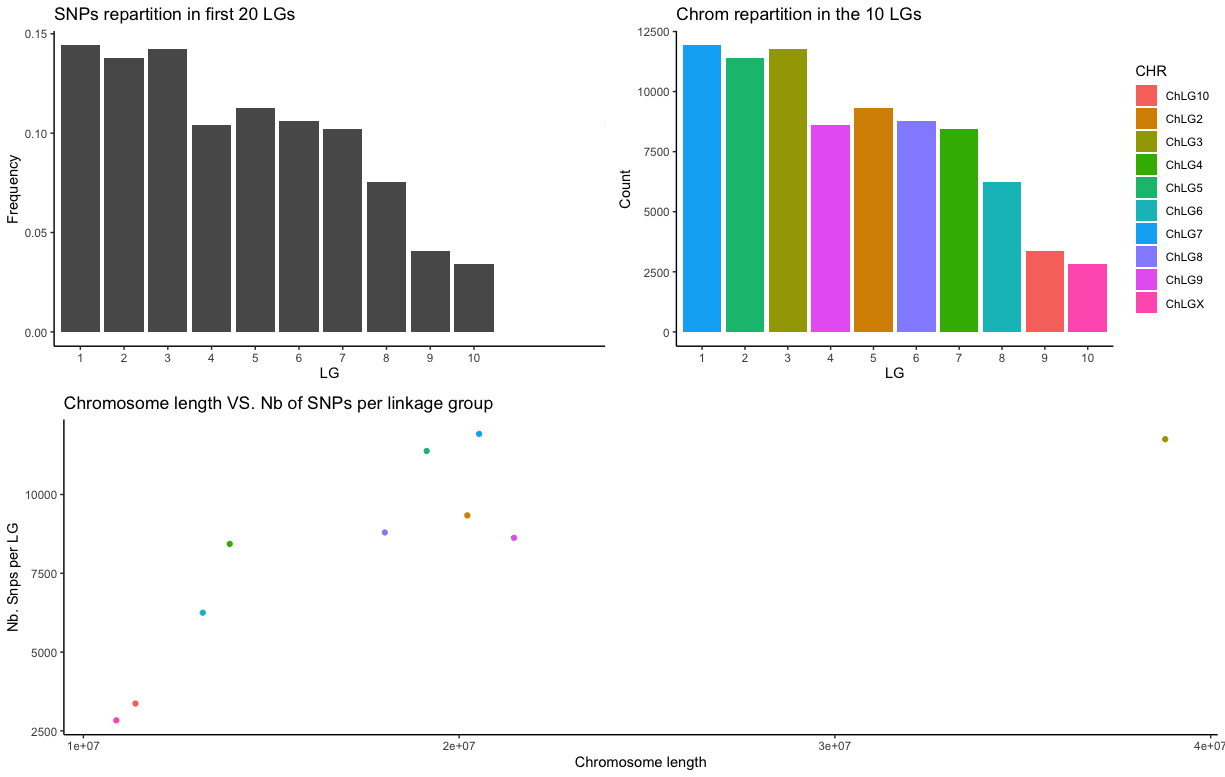
\includegraphics[width=1\linewidth]{figure5.png}
\end{figurehere}

\subsection{OrderMarkers2}

The function \texttt{OrderMarkers2} is called with the following parameters:
\begin{itemize}
\item \texttt{outputPhasedData = 1};
\item \texttt{sexAveraged = 1};
\item \texttt{numThreads = 10};
\end{itemize}

\subsection{Manual cut of map ends for each chromosome}

Genetic distance inflation is observed at both ends of each chromosome map (figure 6).

\hfill

\begin{figurehere}
\centering
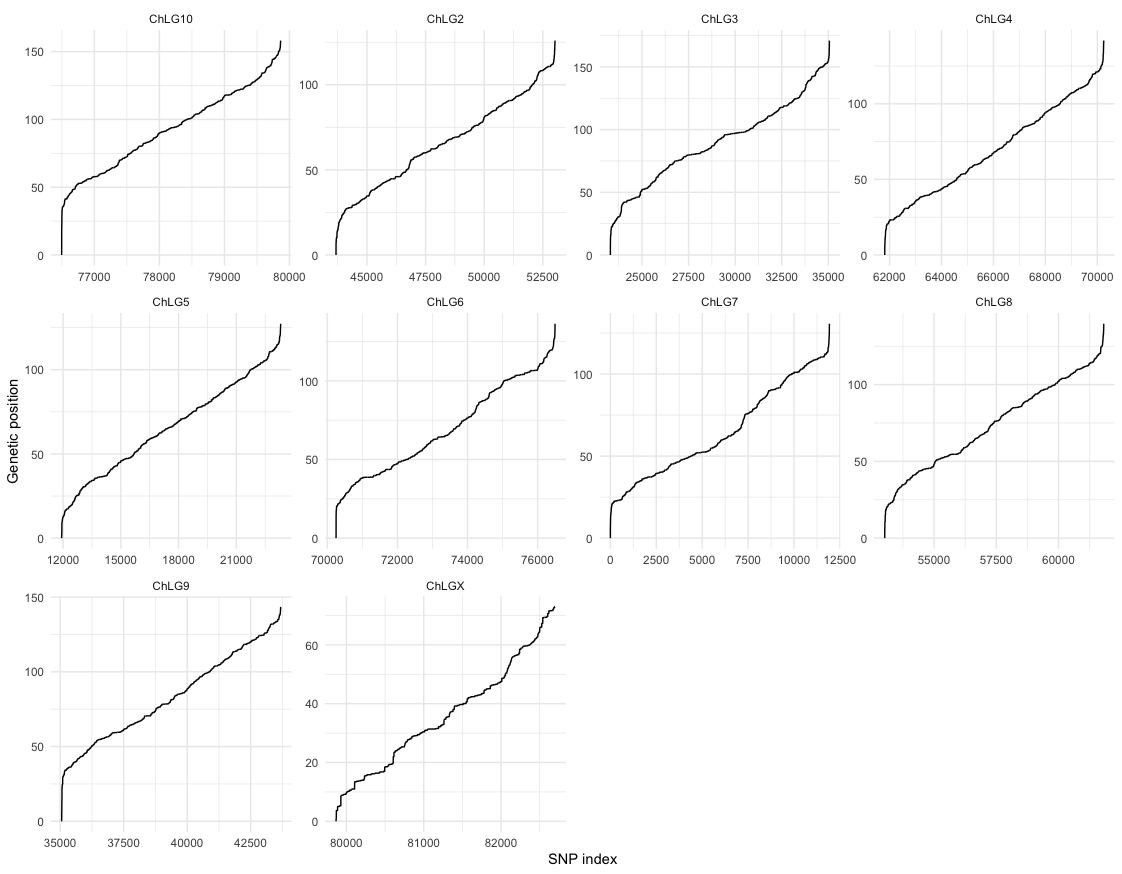
\includegraphics[width=0.51\linewidth]{figure6.png}
\caption{\small{Raw genetic map with genetic distance inflation at chromosome ends.}}
\end{figurehere}

\hfill

Thresholds are applied on each chromosome based on the visual interpretation of Marey maps (figure 7).
Cutoff thresholds are applied on physical and genetic distances, following the table 1. The resulting Marey map is shown on figure 8, and indicates that physical positions from the reference genome correspond well to predicted genetic distances (figure 8).

\hfill

\begin{table}[]
\centering
\caption{\small{List of cutoff values at map ends for each chromosome.}}
\begin{tabular}{l|l|l}
\hline
Chromosome & Genetic distance cutoffs (cM) & Physical distance cutoffs (bp) \\ \hline
ChLGX      & $\varnothing$                 & $\varnothing$                  \\
ChLG2      & $29 < d < 87$                 & $3\times10^6< d <2\times10^7$  \\
ChLG3      & $50 < d < 145$                & $\varnothing$                  \\
ChLG4      & $42< d <110$                  & $d <1.2\times10^7$             \\
ChLG5      & $36< d <101$                  & $\varnothing$                  \\
ChLG6      & $37< d <100$                  & $\varnothing$                  \\
ChLG7      & $37< d <100$                  & $\varnothing$                  \\
ChLG8      & $48< d <100$                  & $\varnothing$                  \\
ChLG9      & $55< d <120$                  & $5\times10^6< d$               \\
ChLG10     & $60< d <125$                  & $2.5\times10^6< d$            
\end{tabular}
\end{table}

\hfill

\begin{figurehere}
\centering
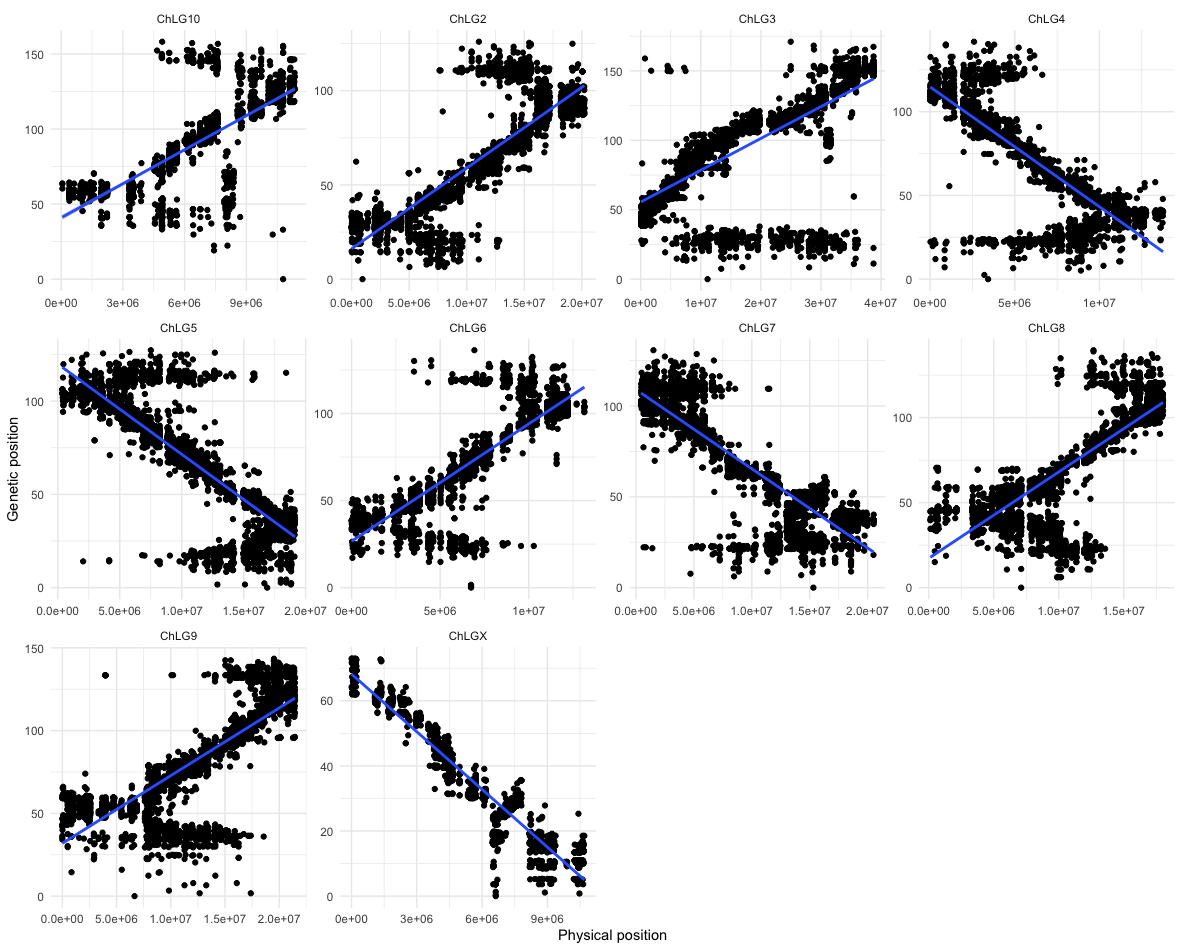
\includegraphics[width=1\linewidth]{figure7.png}
\caption{\small{Marey maps before cutting chromosome ends.}}
\end{figurehere}

\hfill

\begin{figurehere}
\centering
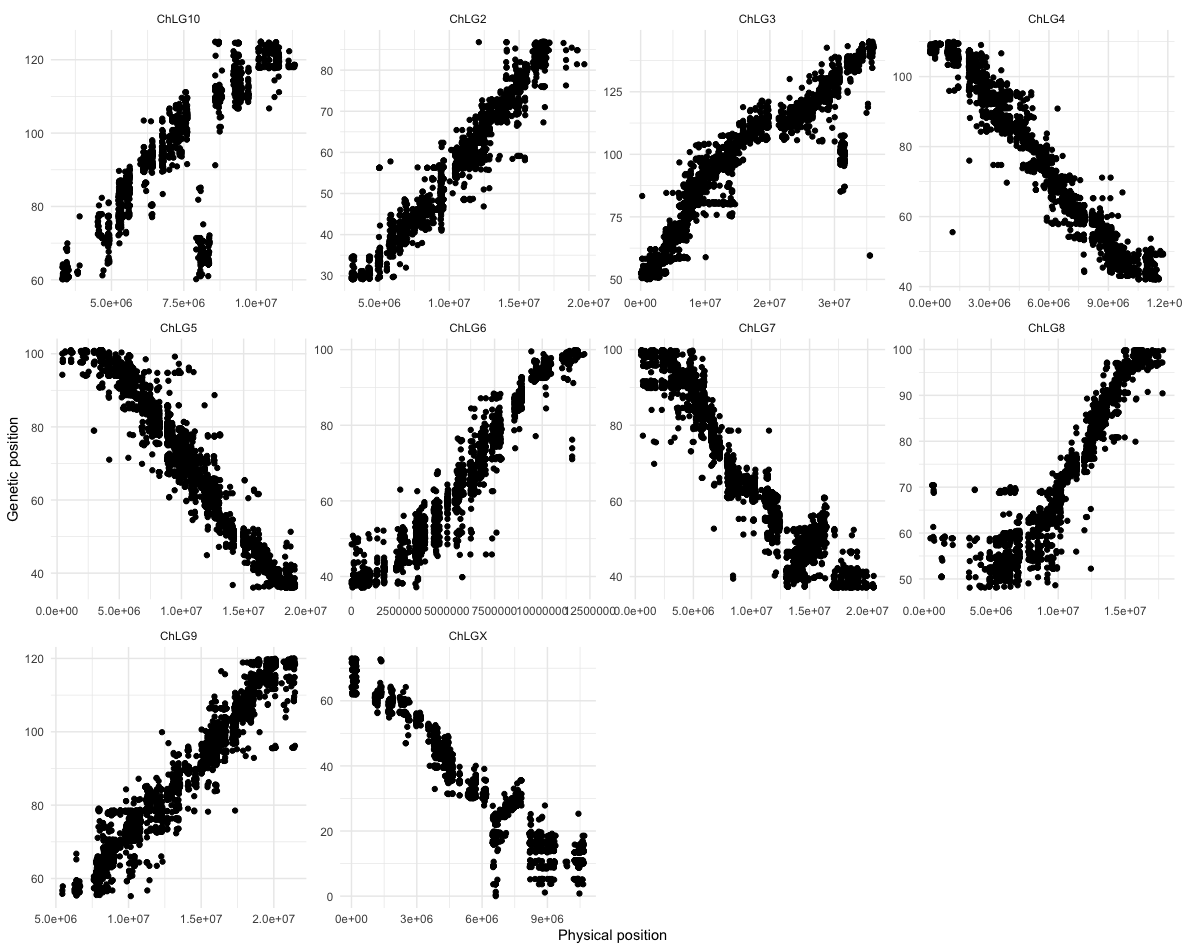
\includegraphics[width=1\linewidth]{figure8.png}
\caption{\small{Marey maps after cutting chromosome ends.}}
\end{figurehere}

%%%%%%%%%%%%%%%%%%%%%%%%%%%
%%%%%%%%%%%%%%%%%%%%%%%%%%%

\bibliographystyle{apalike}
\bibliography{./bibliography.bib}

\end{document}











